\chapter{PENGUJIAN}
\label{sec:chap4_pengujian}
\vspace{1ex}

\section*{}
Pada penelitian ini dipaparkan hasil dari proses yang dipaparkan pada bab 3 serta analisa yang dilakukan sesuai 
dengan desain sistem yang sudah dirancang pada bab sebelumnya. Pembahasan hasil penelitian dilakukan
dengan beberapa bagian seperti berikut :

\begin{itemize}[nolistsep]
    \item Hasil dari Pembuatan Dataset
    \item Hasil \textit{Preprocessing} Data.
    \item Hasil Ekstraksi Fitur.
    \item Hasil Pembelajaran Mesin Mask R-CNN.
    \item Hasil Model Akhir Mask R-CNN.
\end{itemize}

Bagian pertama ialah membahas mengenai hasil dari pembuatan dataset, pada bagian ini akan dijelaskan mengenai
jumlah anotasi objek yang dibentuk. Kemudian pada bagian \textit{preprocessing}, akan dijelaskan hasil mengenai
pembuatan \textit{bounding box}, dan \textit{mini mask}. Kemudian pada bagian ekstraksi fitur dan hasil pembelajaran
mesin Mask R-CNN akan membahas mengenai \textit{pipeline} dari algoritma \textit{Mask R-CNN} secara kesuluruhan.
Kemudian terakhir pada bagian hasil model akhir Mask R-CNN akan dijelaskan mengenai 

\section{Hasil Pembuatan Dataset}
Pengambilan data video dilakukan di Pasar Atom pada bulan Januari 2022 dimana total video yang dikumpulkan adalah 24 menit
dan terdiri dari 6 lokasi. Pengambilan data dilakukan pada jam 1 hingga 2 siang. Setelah pengambilan video dilakukan,
1 frame setiap 90 frame pada video diekstrak sehingga menghasilkan 730 gambar. Gambar-gambar ini kemudian dibagi
menjadi tiga set (\textit{train set, test set} dan \textit{val set}) dengan perbandingan 0.6 : 0.2 : 0.2.
\textit{Train set} memiliki total gambar 436 gambar, \textit{test set} memiliki total 146 gambar, dan sama
seperti \textit{test set}, val set juga memiliki 146 gambar. Kemudian pada setiap gambar tersebut, objek manusia
dibedakan menjadi tiga kelompok atau kelas. Seperti yang sudah dijelaskan pada bab sebelumnya, kelas tersebut ialah

\begin{itemize}
    \item Kelas \textit{Person}, dimana objek manusia tersebut berada sendirian pada radius satu meter dapat dilihat
    pada gambar \ref{fig: Kelas Person}.
    \item Kelas \textit{Group}, dimana terdapat dua hingga tiga orang yang berada pada radius satu meter dapat dilihat
    pada gambar \ref{fig: Kelas Group}.
    \item Kelas \textit{Crowd}, dimana terdapat empat orang atau lebih yang berada berdekatan pada jarak radius
        satu meter dapat dilihat pada gambar \ref{fig: Kelas Crowd}.
\end{itemize}

\begin{figure}[h!]
    \begin{center}
      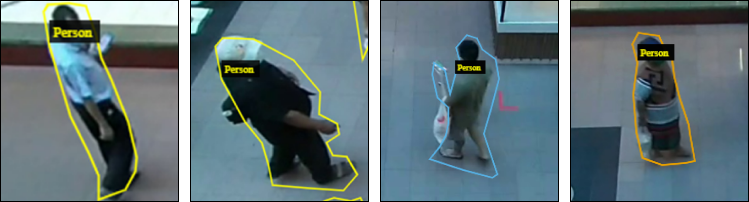
\includegraphics[width= 0.8\linewidth]{bab4/Person_class_2.png}
      \caption{Contoh Kelas \textit{Person}}
      \label{fig: Kelas Person}
    \end{center}
\end{figure}

\begin{figure}[h!]
    \begin{center}
      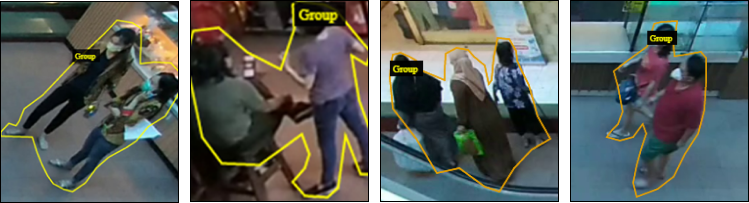
\includegraphics[width= 0.8\linewidth]{bab4/Group_class_2.png}
      \caption{Contoh Kelas \textit{Group}}
      \label{fig: Kelas Group}
    \end{center}
\end{figure}

\begin{figure}[h!]
    \begin{center}
      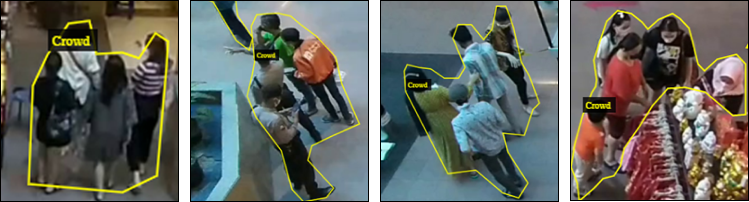
\includegraphics[width= 0.8\linewidth]{bab4/Crowd_class_2.png}
      \caption{Contoh Kelas \textit{Crowd}}
      \label{fig: Kelas Crowd}
    \end{center}
\end{figure}

Total objek yang dianotasi pada seluruh 730 gambar adalah 4.980 objek yang terdiri dari 3.382 objek kelas 
\textit{person}, 1.350 kelas \textit{group}, dan 248 kelas \textit{crowd}. Sedangkan jika dibagi pada tiap set,
\textit{Train set} memiliki 2.054 objek kelas \textit{person}, 732 objek kelas \textit{group}, dan 159 objek
kelas \textit{crowd}. \textit{Test set} memiliki 687 objek kelas \textit{person}, 321 objek kelas \textit{group},
dan 40 objek kelas \textit{crowd}. Sedangkan pada \textit{val set} memiliki 641 objek kelas \textit{person}, 
297 objek kelas \textit{group}, dan 49 objek kelas \textit{crowd}. Dapat dikatakan bahwa dataset ini merupakan
dataset yang tidak seimbang (\textit{imbalance dataset}) namun dalam kondisi Covid-19, objek kerumunan memang lebih
jarang ditemukan dibandingkan objek \textit{person} atau orang yang menjaga jarak satu sama lain. Tentunya hal ini
juga dapat digunakan untuk melihat perilaku para pengunjung, penjual, maupun petugas saat kondisi Covid-19. Dataset
ini juga dapat membantu penelitian lain dalam mengembangkan suatu program deteksi kerumunan terutama dalam pusat 
perbelanjaan.

\begin{table}[h]
    \caption{Detail Jumlah Objek Anotasi}
    \label{tab:specs_collab}
    \centering
    \begin{tabular}{|l|l|l|l|}
        \hline
        \textbf{Set}                    & Kelas \textit{Person} & Kelas \textit{Group} & Kelas \textit{Crowd}   \\ \hline
        \textit{\textbf{Train Set}}      & 2.054 & 732 & 159        \\ \hline
        \textit{\textbf{Test Set}}     & 687 & 321 & 40             \\ \hline
        \textit{\textbf{Val Set}}       & 641 & 297 & 49            \\ \hline
    \end{tabular}
\end{table}

\begin{figure}[h!]
    \begin{center}
      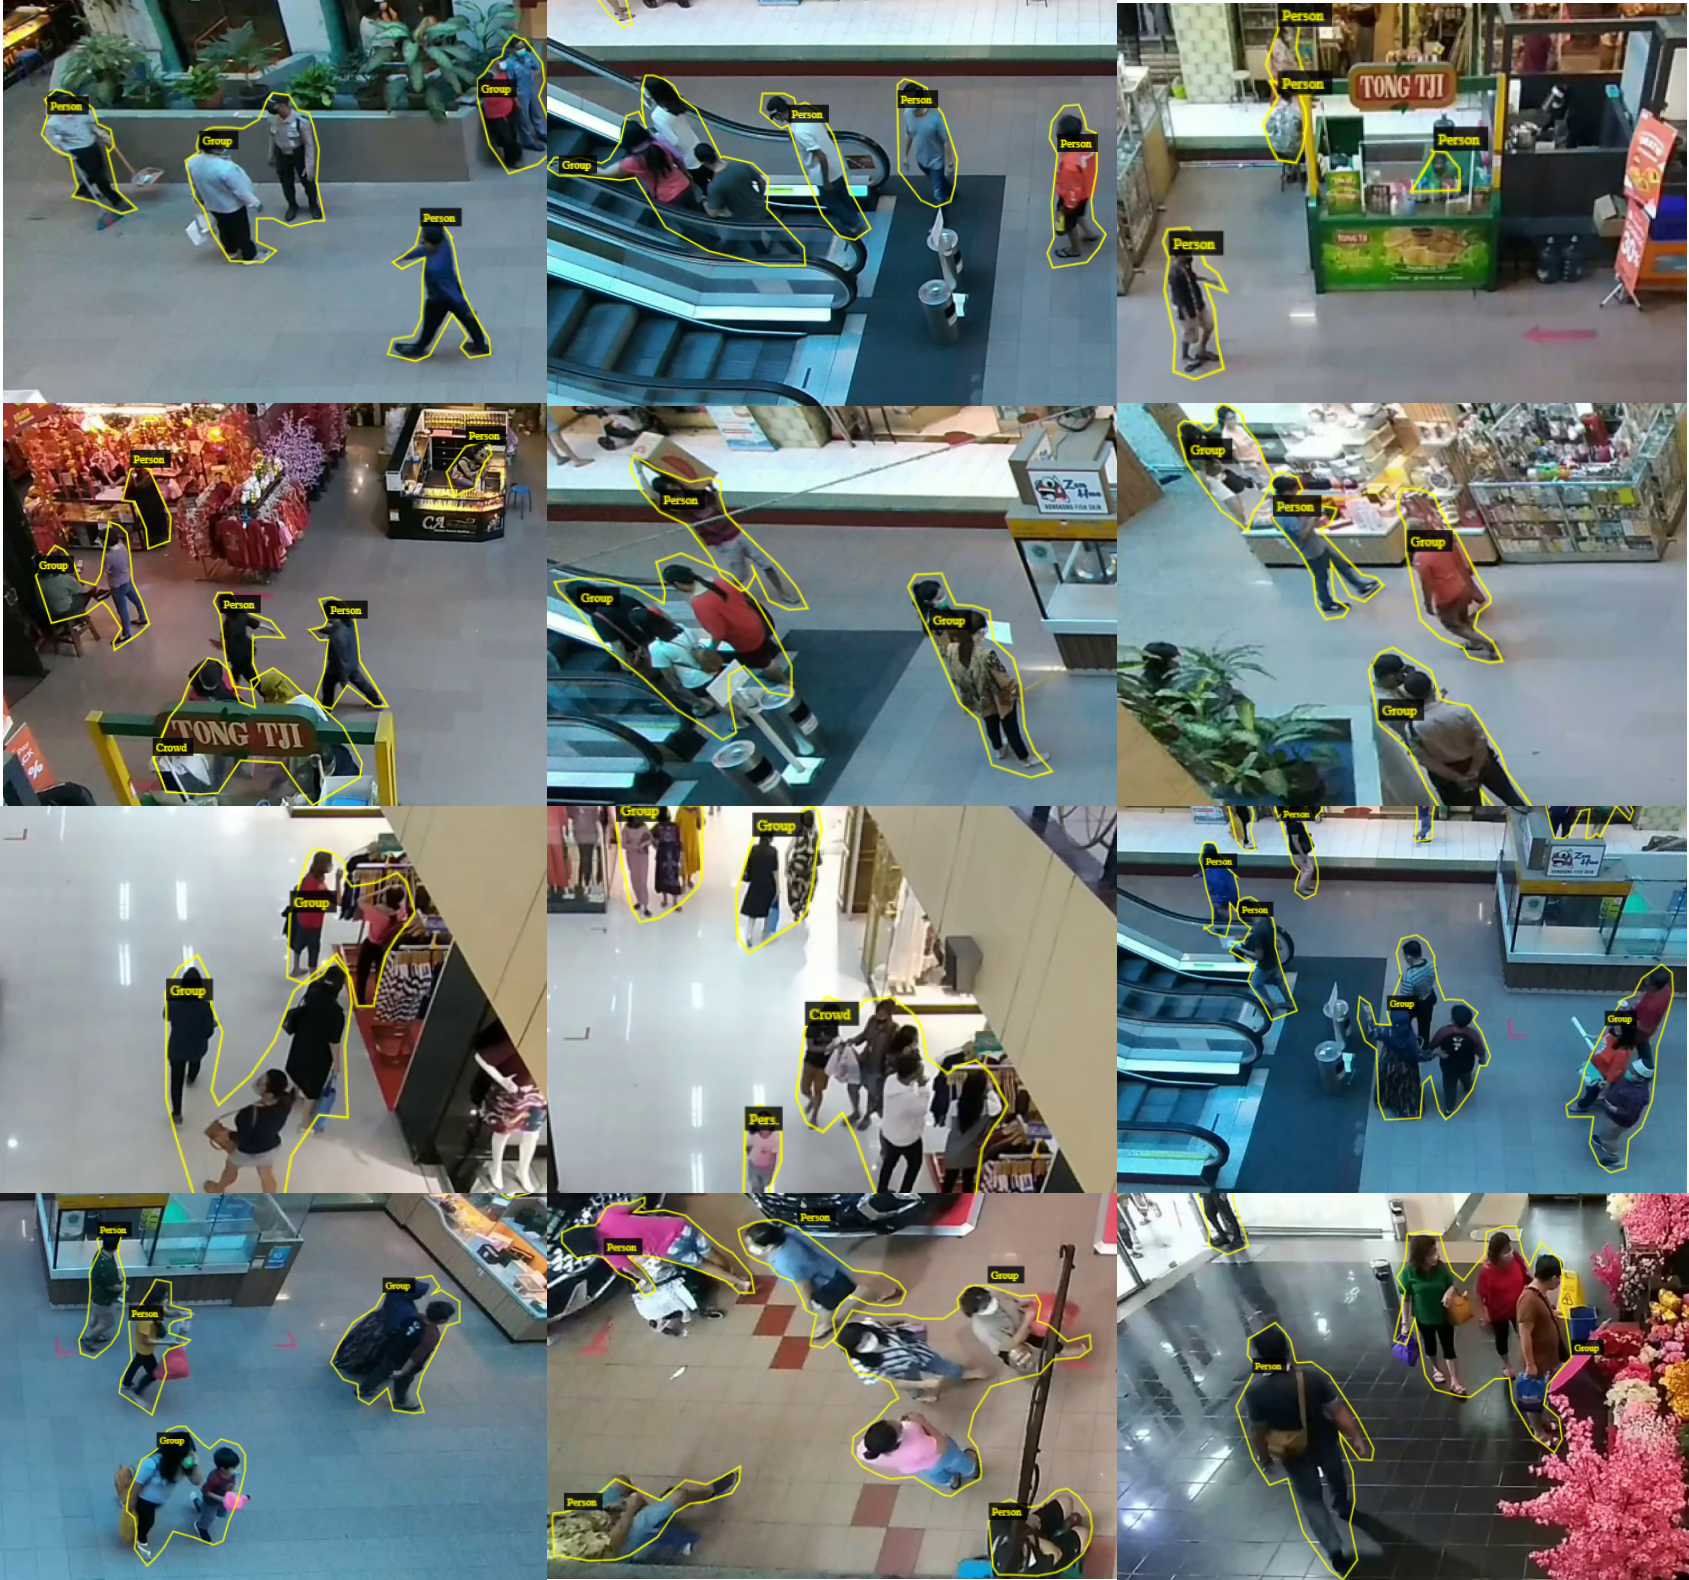
\includegraphics[width= 0.8\linewidth]{bab4/Dataset.png}
      \caption{Contoh Beberapa Hasil Dataset}
      \label{fig: Dataset}
    \end{center}
\end{figure}

\section{Hasil \textit{Preprocessing} Data}
Pada bagian ini, hasil mengenai \textit{preprocessing data pipeline} pada dataset yang telah dibentuk akan dijelaskan
secara lebih mendalam. 

\subsection{Hasil Pembuatan \textit{Bounding Box}}
Seperti yang telah dijelaskan sebelumnya pada bab metodologi, pembuatan \textit{bounding box} dilakukan dengan
mengikuti ukuran dari \textit{mask}. Jumlah \textit{bounding box} pada tahap ini mempunyai nilai yang sama dengan
jumlah objek pada dataset yaitu 4.970 objek.

\begin{figure}[h!]
  \begin{center}
    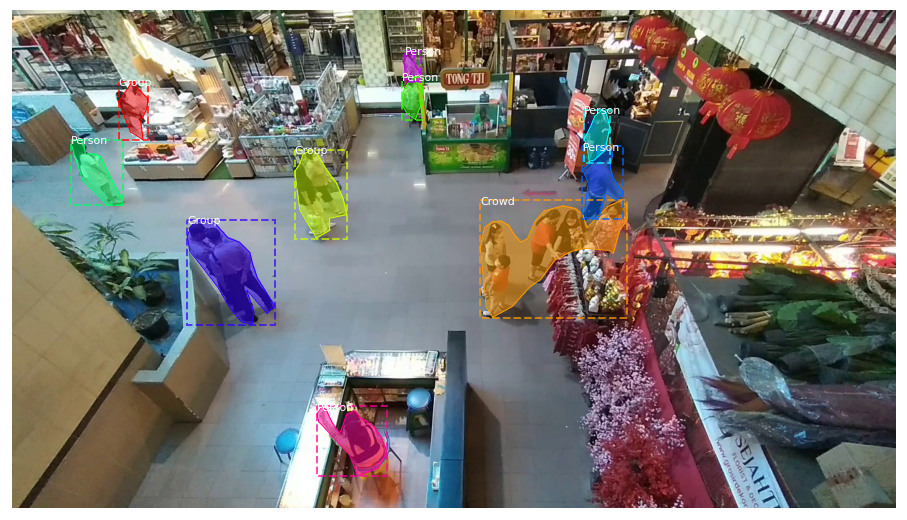
\includegraphics[width= 0.8\linewidth]{bab4/Contoh Bounding Box.png}
    \caption{Contoh Hasil Pembuatan \textit{Bounding Box}}
    \label{fig: Contoh Bounding Box}
  \end{center}
\end{figure}

\subsection{Hasil Pengubahan Ukuran Gambar}
Setelah koordinat \textit{bounding box} didapatkan dan \textit{bounding box} dapat dibentuk, maka ukuran gambar akan
disamakan sesuai dengan input pada model dimana pada penelitian ini ialah 1024 x 1024 piksel. Ukuran gambar yang awalnya
berukuran 1920 x 1080 dirubah menjadi 1024 x 1024 dengan cara memperkecil ukuran gambar dan memberikan piksel
hitam pada bagian atas dan bawah gambar. Hasil dari \textit{preprocess} ini dapat dilihat pada gambar 
\ref{fig: Contoh Resize Image}. Dimensi gambar pun berubah menjadi 1024 x 1024 x 3. Pada penelitian  ini
fitur warna tetap digunakan sebagai fitur, walaupun mungkin dalam kenyataannya, dimensi warna ini dapat dirubah
menjadi satu jenis saja.

\begin{figure}[h!]
  \begin{center}
    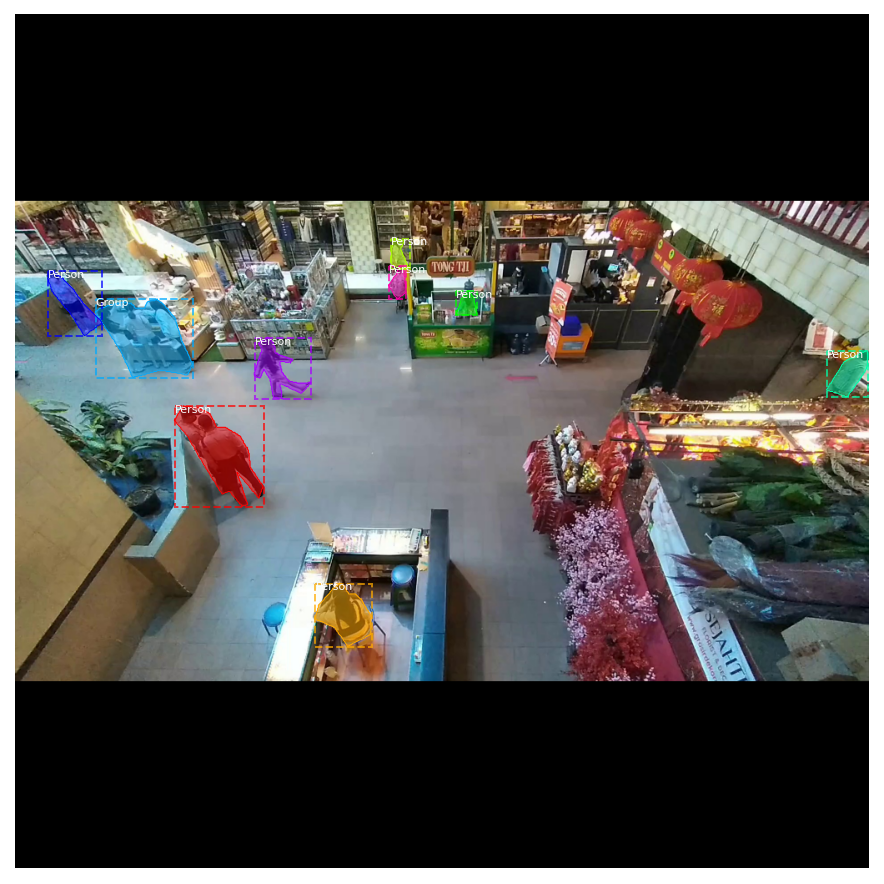
\includegraphics[width= 0.65\linewidth]{bab4/Resize Image.png}
    \caption{Contoh Hasil \textit{Resizing} Image}
    \label{fig: Contoh Resize Image}
  \end{center}
\end{figure}


\subsection{Hasil Pembuatan \textit{Mini Mask}}
Setelah gambar-gambar dataset mempunyai ukuran yang sama dan sesuai dengan input dari model, maka hal selanjutnya
yang perlu dilakukan ialah pembentukan \textit{mini mask}. Sebelumnya, \textit{mask} yang terbentuk pada dataset
juga mempunyai ukuran yang sama pada gambar, tentunya hal ini tidak efektif karena \textit{mask} tersbeut dibedakan
sesuai objeknya dan mempunyai banyak nilai null. Karena itu, bentuk \textit{mask} diubah menjadi ukuran 56 x 56 piksel.

\begin{figure}[h!]
  \begin{center}
    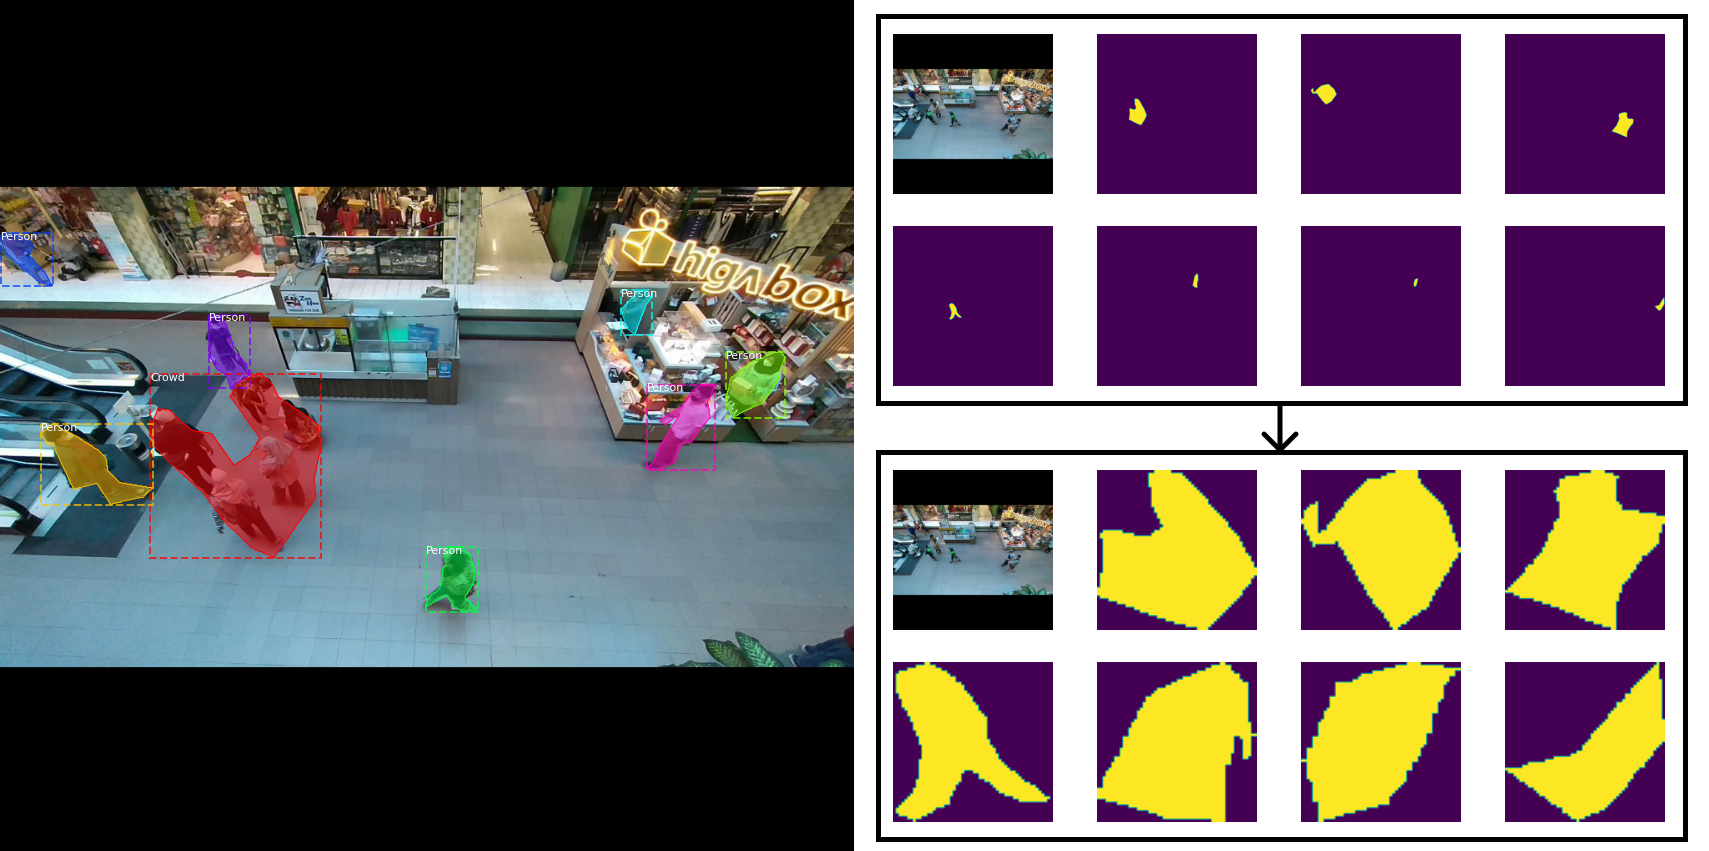
\includegraphics[width= 0.8\linewidth]{bab4/Mini Mask.png}
    \caption{Contoh Hasil Pembuatan \textit{Mini Mask}}
    \label{fig: Contoh Mini Mask}
  \end{center}
\end{figure}

\section{Hasil \textit{Feature Extraction}}
Pada bagian ini, hasil mengenai \textit{feature extraction pipeline} pada dataset yang telah di-\textit{preprocess}
akan dijelaskan secara lebih mendalam. Proses \textit{feature extraction} yang dilakukan pada tahap ini sudah
menggunakan algoritma Mask-RCNN. Namun hasil yang dikemukakan pada bagian ini adalah hasil \textit{feature map}.
Sedangkan hasil mengenai proses Mask R-CNN yang memberikan klasifikasi kelas, \textit{bounding box}, dan membangkitkan
\textit{mask}.

\begin{figure}[h!]
    \begin{center}
      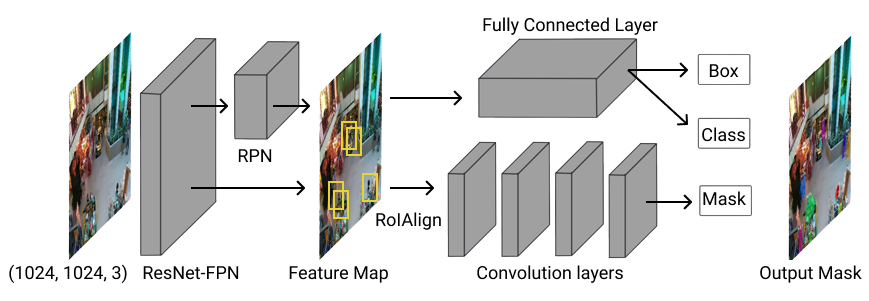
\includegraphics[width= 0.8\linewidth]{bab4/Metodologi_Training_2.png}
      \caption{Arsitektur Mask R-CNN yang diaplikasikan}
      \label{fig: Crowd Mask RCNN Archi}
    \end{center}
\end{figure}

Sesuai dengan proses algoritma Mask R-CNN yang diilustrasikan pada gambar \ref{fig: Crowd Mask RCNN Archi}
Proses Mask R-CNN dimulai dengat ekstraksi fitur pada jaringan \textit{backbone} dimana pada penelitian ini
\textit{backbone} yang digunakan ialah ResNet 101. Kemudian hasil dari ResNet akan menghasilkan prediksi
RPN \textit{Regional Proposal Network} serta \textit{feature map} yang merupakan hasil dari konvolusi dan
\textit{pooling} pada jaringan ResNet, kemudian pada \textit{feature map} tersebut akan diproses oleh
\textit{fully connected layer} untuk melakukan prediksi mengenai \textit{bounding box} pada objek serta
kelas daripada objek tersebut. Selain itu \textit{convolution layer} akan menggunakan fitur-fitur pada 
\textit{feature map} untuk membentuk \textit{mask} dari objek. Hasil \textit{training} dari pemprosesan
oleh \textit{Fully Connected Layer} dan \textit{Convolution Layer} akan dijelaskan pada subbab berikutnya.

\subsection{Hasil \textit{Pembuatan Anchor Box}}
Bagian pertama pada proses \textit{feature extraction} adalah membuat \textit{anchor box} yang akan digunakan
untuk target RPN. Untuk penentuan \textit{anchor box} yang akan menjadi target RPN, maka digunakan metriks IoU
\textit{Intersect over Union}, jika \textit{bounding box ground} atau \textit{bounding box} asli memiliki IoU lebih
dari sama dengan 0.7 dengan \textit{anchor box}, maka \textit{anchor box} tersebut digunakan sebagai target RPN.
Hasil dari pembuatan \textit{anchor box} ditunjukkan pada gambar \ref{fig: Anchor Box}. Sedangkan contoh 
\textit{anchor box} yang digunakan sebagai target RPN dapat dilihat pada gambar \ref{fig: Anchor Box Positive}.
Untuk menunjukkan adanya perbedaan mengenai \textit{anchor box} yang digunakan sebagai target dan dengan
yang tidak maka hasil \textit{anchor box} yang tidak digunakan pada proses melatih jaringan \textit{backbone} dalam
memprediksi RPN juga ditampilkan dan dapat dilihat pada \ref{fig: Anchor Box Negative}.

\begin{figure}[h!]
  \begin{center}
    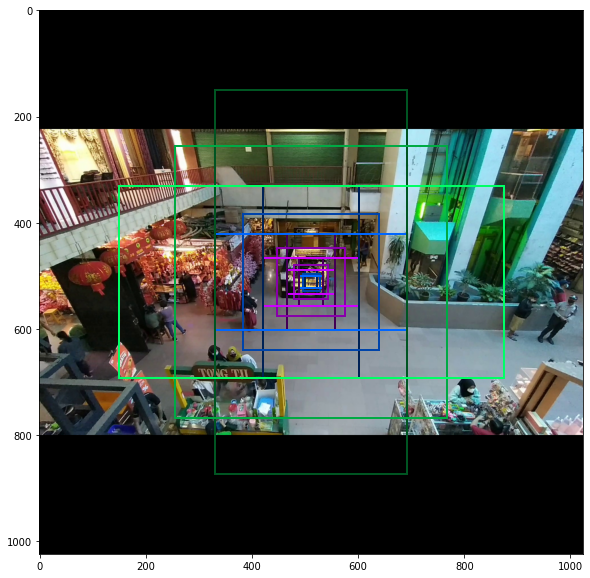
\includegraphics[width= 0.55\linewidth]{bab4/Anchor Box.png}
    \caption{Hasil \textit{Anchor Box} yang Dihasilkan}
    \label{fig: Anchor Box}
  \end{center}
\end{figure}

\begin{figure}[h!]
  \begin{center}
    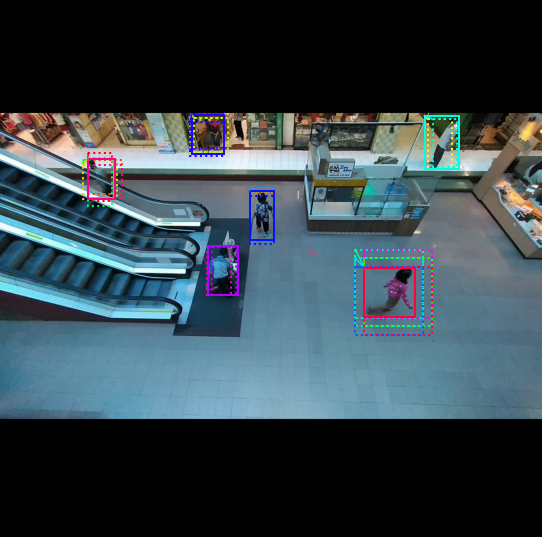
\includegraphics[width= 0.5\linewidth]{bab4/Anchor Box Positive.png}
    \caption{Contoh Hasil \textit{Anchor Box} yang Menjadi Target RPN}
    \label{fig: Anchor Box Positive}
  \end{center}
\end{figure}

\begin{figure}[h!]
  \begin{center}
    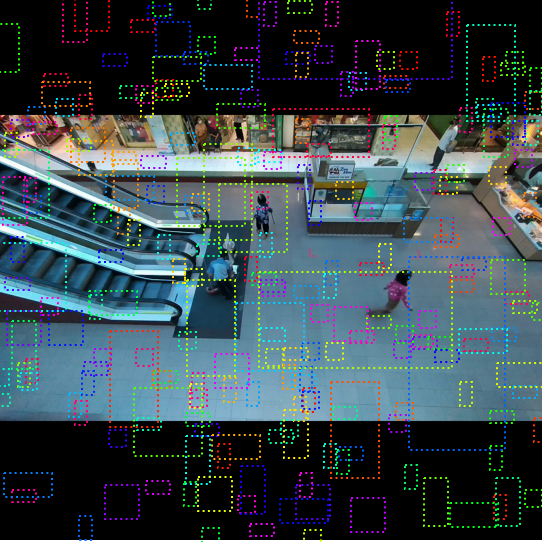
\includegraphics[width= 0.45\linewidth]{bab4/Anchor Box Negative.png}
    \caption{Contoh Hasil \textit{Anchor Box} yang Tidak Digunakan}
    \label{fig: Anchor Box Negative}
  \end{center}
\end{figure}

\subsection{Hasil Prediksi RPN dan Pembuatan \textit{Feature Map}}
Setelah jaringan \textit{residual network} dilatih menggunakan target RPN, maka prediksi RPN pun dapat dilakukan
oleh ResNet. Prediksi RPN dilakukan dengan menggunakan \textit{train-set} dan \textit{val-set} sehingga performa
model dapat diketahui secara lebih dalam terutama dalam mengidentifikasi adanya \textit{overfitting} maupun
\textit{underfitting}. RPN ini juga akan turut serta membantu dalam membentuk \textit{feature map} karena
jaringan ResNet ingin memperlihatkan fitur-fitur pada \textit{regional proposal network} yang telah diprediksi
dengan konvolusi dan \textit{pooling}. Pada tahap ini, RPN juga mendeteksi kelas pada objek di dalam \textit{bounding box}
namun deteksi kelas yang dimaksud ialah deteksi apakah objek tersebut termasuk \textit{foreground} atau 
\textit{background}. Dalam memprediksi kelas objek, \textit{loss} yang terjadi pada rpn umumnya bernilai
kecil karena hanya memprediksi dua nilai saja yaitu \textit{foreground} atau \textit{background}.

\begin{figure}[h!]
  \begin{center}
    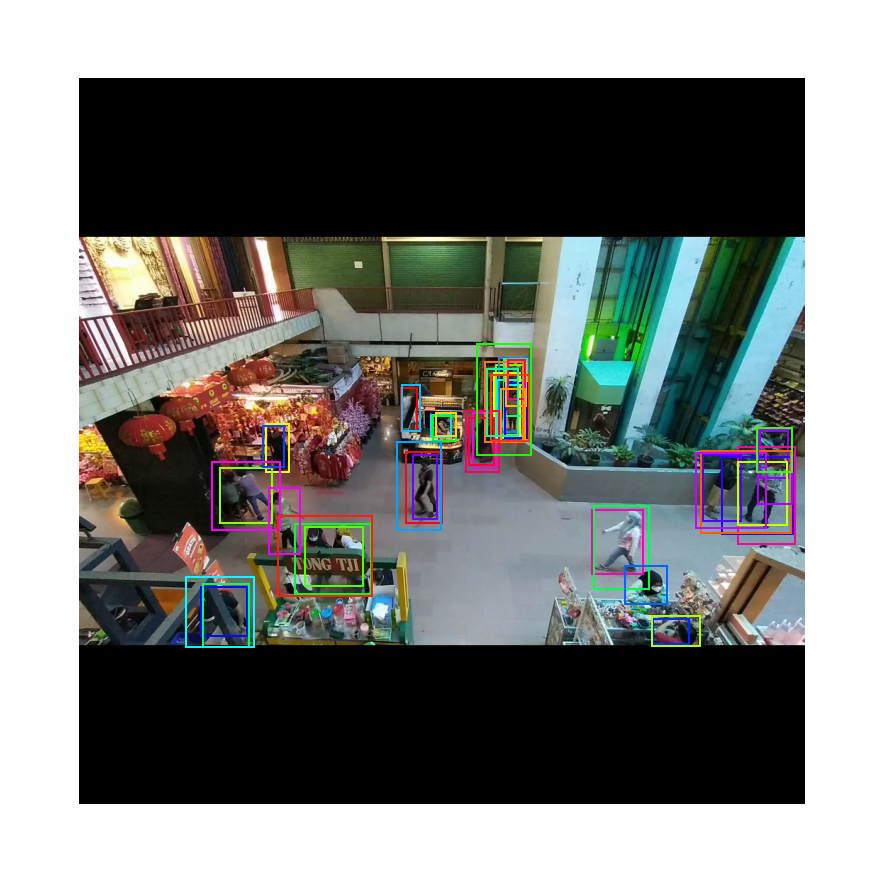
\includegraphics[width= 0.5\linewidth]{bab4/Prediksi RPN.png}
    \caption{Contoh Hasil Prediksi RPN}
    \label{fig: Prediksi RPN}
  \end{center}
\end{figure}

\begin{figure}[h!]
  \begin{center}
    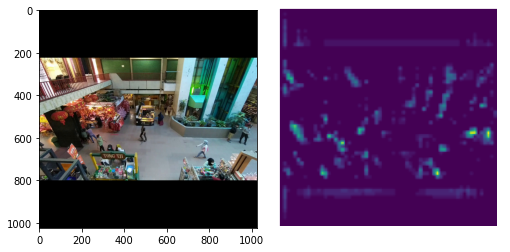
\includegraphics[width= 0.55\linewidth]{bab4/Feature Map Example.png}
    \caption{Contoh Hasil \textit{Feature Map}}
    \label{fig: Feature Map}
  \end{center}
\end{figure}

\subsection{Hasil \textit{Training}}
Pada bagian ini akan dijelaskan secara lebih mendalam mengenai hasil dari model yang telah dibentuk. 
Beberapa metriks \textit{loss} yang dipaparkan adalah sebagai berikut.

\begin{itemize}
  \item \textbf{\textit{Loss}} 
  
  Metriks \textit{loss} merupakan metriks yang menunjukkan jumlah dari segala \textit{loss} yang terjadi pada
  pemodelan, sedangkan \textit{val loss} adalah jumlah \textit{loss} yang terjadi saat model
  diuji coba pada dataset validasi.

  \item \textbf{\textit{RPN Bounding Box Loss}} 
  
  Metriks \textit{loss} mengenai \textit{bounding box} yang terjadi pada RPN menunjukkan adanya
  kesalahan prediksi pada jaringan \textit{backbone} dalam memprediksi \textit{bounding box} yang
  sesuai seperti target RPN. Kesalahan prediksi ditunjukkan dengan jauhnya jarak \textit{anchor box} asli
  dengan \textit{bounding box} yang diprediksi. Hasil \textit{RPN Bounding Box Loss} dari proses \textit{training} dapat dilihat pada gambar
  \ref{fig: RPN Bounding Box Loss Mask RCNN}.

  \item \textbf{\textit{RPN Class Loss}} 
  
  Sedangkan Metriks \textit{RPN Class loss} menunjukkan adanya kesalahan prediksi pada RPN
  untuk membedakan \textit{foreground} dan \textit{background} pada objek atau citra yang berada
  pada di dalam \textit{bounding box} yang telah diprediksi, nilai \textit{loss} ini umumnya bernilai
  lebih kecil daripada \textit{loss} yang lain karena hanya kesalahan prediksi untuk membedakan 
  dua kelas. Hasil \textit{RPN Class Loss} dari proses \textit{training} dapat dilihat pada gambar
  \ref{fig: RPN Class Loss}.

  \item \textbf{\textit{Mask RCNN Bounding Box Loss}} 
  
  Metriks \textit{Mask RCNN Bounding Box Loss} mengenai \textit{bounding box} yang terjadi pada 
  \textit{fully connected layer}. Hampir sama dengan metriks \textit{RPN Bounding Box Loss}, 
  kesalahan prediksi ditunjukkan dengan jauhnya jarak \textit{anchor box} asli
  dengan hasil akhir \textit{bounding box} yang diprediksi. Hasil \textit{Mask RCNN Bounding Box Loss} 
  dari proses \textit{training} dapat dilihat pada gambar \ref{fig: Bounding Box Loss Mask RCNN}.

  \item \textbf{\textit{Mask RCNN Class Loss}} 
  
  Metriks \textit{Mask RCNN Class Loss} memberikan penilaian mengenai kesalahan prediksi kelas,
  dimana pada penelitian ini, \textit{Mask RCNN Class Loss} akan bertambah jika Mask RCNN 
  memberikan kesalahan klasifikasi antara tiga kelas objek. Hasil \textit{Mask RCNN Class Loss} 
  dari proses \textit{training} dapat dilihat pada gambar \ref{fig: Class Loss Mask RCNN}.

  \item \textbf{\textit{Mask RCNN Mask Loss}}
  
  Metriks \textit{Mask RCNN Mask Loss} memberikan penilaian mengenai kesalahan pembentukan 
  \textit{mask} objek. Jika \textit{mask} yang dibentuk oleh model mempunyai selisih yang jauh dengan
  \textit{mask} yang dibentuk di awal, maka nilai \textit{Mask RCNN Mask Loss} akan bertambah.
  Hasil \textit{Mask RCNN Class Loss} dari proses \textit{training} dapat dilihat pada gambar 
  \ref{fig: Mask Loss Mask RCNN}.

\end{itemize}

Dalam pemilihan model terbaik yang dapat diaplikasikan, metriks \textit{val loss} merupakan yang
terbaik karena metriks tersebut mencerminkan bagaiman model Mask R-CNN bekerja pada data yang belum pernah
dilihat sebelumnya. Dari grafik-grafik \textit{loss} yang dipaparkan, dapat diperhatikan bahwa 
pada epoch 0 hingga 60, nilai \textit{loss} dan \textit{val loss} menunjukkan penurunan yang signifikan,
sedangkan pada epoch 60 hingga 150, nilai \textit{loss} tetap menurun, namun nilai \textit{val loss}
tidak menunjukkan adanya perubahan yang signifikan. Hal ini dapat dikarenakan kecilnya \textit{learning rate}
yang diaplikasikan atau karena model telah mencapai nilai optimal.
Nilai \textit{val loss} mencapai titik terendah pada epoch 124 dengan nilai 0,772 dan nilai 
\textit{loss} 0,5877. Karena nilai \textit{val loss} pada 
model epoch 124 mempunyai nilai terkecil, maka model inilah yang akan diteliti lebih lanjut dan diuji
coba pada test dataset. Namun sebelum itu, parameter \textit{loss} yang lain perlu dilihat untuk
memastikan apakah proses \textit{training} berjalan dengan baik. 

\begin{figure}[h!]
  \begin{center}
    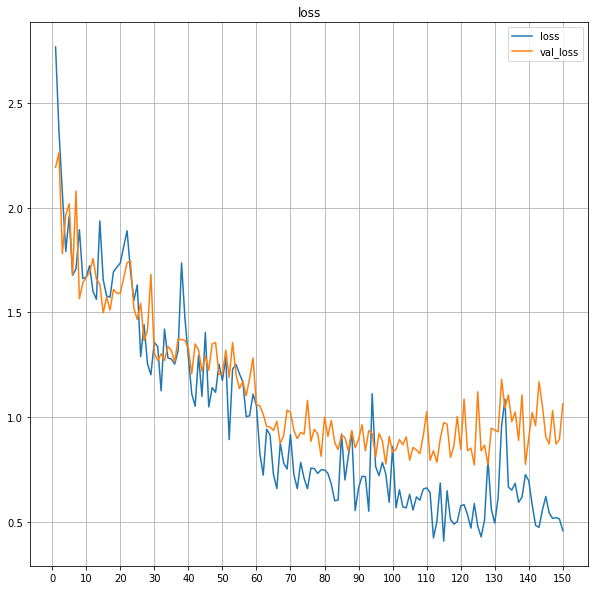
\includegraphics[width= 0.55\linewidth]{bab4/1. Loss_Result.png}
    \caption{Hasil \textit{Loss}}
    \label{fig: Loss}
  \end{center}
\end{figure}

Selain memberikan informasi mengenai nilai \textit{val loss} terendah, grafik \textit{loss} pada gambar \ref{fig: Loss} menunjukkan adanya \textit{overfitting}. \textit{Overfitting}
dapat diakibatkan oleh banyak faktor seperti arsitektur \textit{neural network}, penggunaan \textit{hyperparameter},
dan kurangnya dataset yang diambil. Dalam penelitian ini, kemungkinan besar hal ini terjadi karena adanya
ketidak seimbangan antara kelas dataset dan kurang dataset kelas \textit{crowd}. Karena itu \textit{overfitting}
terjadi, namun kualitas dari model dapat dilihat terlebih dahulu sehingga dapat diketahui apakah data
yang lebih banyak memang diperlukan, atau performa model dapat diterima walau mengalami \textit{overfitting}.
Selain itu komponen parameter \textit{loss} apakah yang menyebabkan nilai \textit{val loss} tidak mengalami penurunan
juga dapat diketahui jika melihat grafik setiap parameter \textit{loss}.

Selanjutnya pada metriks \textit{RPN Class Loss} (gambar \ref{fig: RPN Class Loss}) dapat dilihat bahwa
nilai \textit{loss} yang terjadi di awal sudah kecil dibandingkan metriks \textit{loss} yang lain. Nilai
awal pada \textit{RPN class loss} adalah 0,07 kemudian mempunyai nilai pada epoch 124 dengan nilai 0,0069.
Sehingga dapat dikatakan bahwa model pada epoch 124 dapat membedakan objek yang menjadi fokus (\textit{foreground})
dan objek yang menjadi latar belakang atau \textit{background}. Proses pembelajaran \textit{ResNet} dalam
membedakan \textit{foreground} maupun \textit{background} dapat terbilang cukup baik karena memiliki
nilai \textit{loss} yang menurun pada epoch 0 hingga 100, namun nilai \textit{loss} mulai berangsur naik
saat epoch lebih dari 100. Di saat inilah \textit{overfitting} mengenai prediksi \textit{foreground} dan
\textit{background} terjadi.

\begin{figure}[h!]
  \begin{center}
    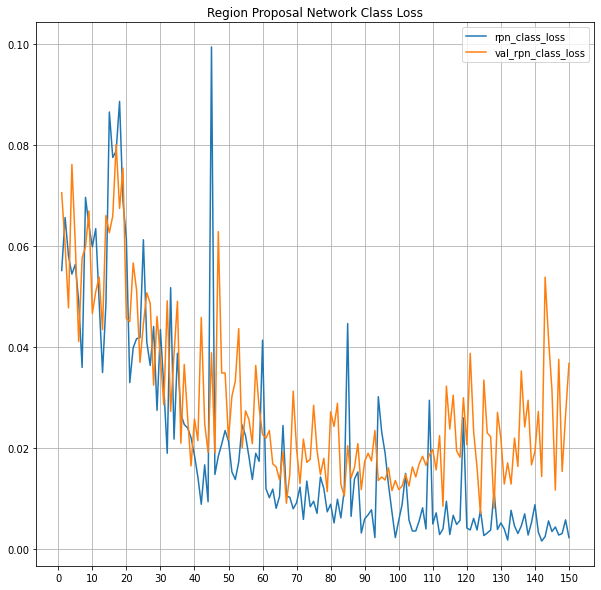
\includegraphics[width= 0.55\linewidth]{bab4/5. RPN_Class_Loss.png}
    \caption{Hasil \textit{Class Loss} RPN}
    \label{fig: RPN Class Loss}
  \end{center}
\end{figure}

Kemudian pada metriks \textit{RPN Bounding Box Loss} (gambar \ref{fig: RPN Bounding Box Loss Mask RCNN})
dapat dilihat bahwa nilai awal pada metriks \textit{loss} adalah 0,45 dan mencapai nilai minimal 0,1591
pada epoch 95. Sedangkan pada epoch 124 yang merupakan model dengan total val loss paling rendah memiliki \textit{val rpn bounding box loss} adalah 0,1921. 
Walaupun bukan nilai terendah, namun selisih nilai \textit{val rpn bounding box loss} epoch 124 mempunyai selisih
yang cukup kecil dengan epoch 95.

\begin{figure}[h!]
  \begin{center}
    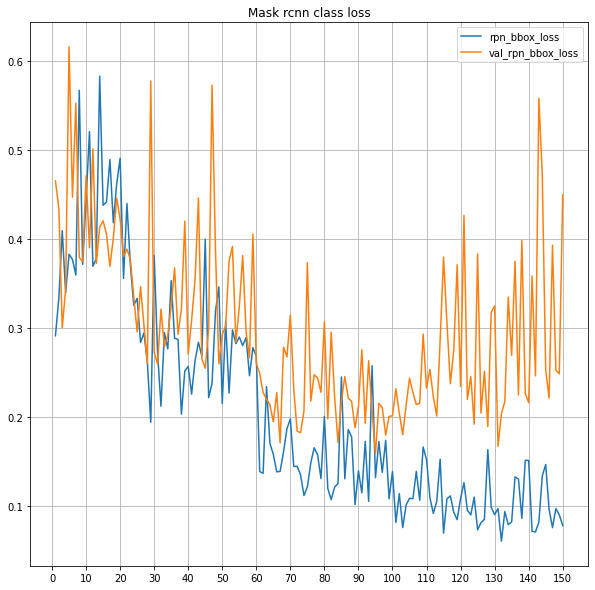
\includegraphics[width= 0.55\linewidth]{bab4/6. RPN_Bbox_Loss.png}
    \caption{Hasil \textit{Bounding Box Loss} RPN}
    \label{fig: RPN Bounding Box Loss Mask RCNN}
  \end{center}
\end{figure}

Selanjutnya pada metriks \textit{class loss Mask RCNN} (gambar \ref{fig: Class Loss Mask RCNN})
dapat dilihat bahwa nilai awal pada metriks \textit{val loss} berada di sekitar 0,7 dan mencapai nilai minimal 0,1032
pada epoch 144. Metriks \textit{class loss Mask RCNN} merupakan parameter yang menunjukkan apakah
Mask R-CNN dapat memprediksi kelas objek dengan benar atau tidak. Dalam melatih kemampuan Mask R-CNN
dalam mendeteksi kelas objek, dapat dilihat bahwa nilai loss kelas memiliki trend yang menurun. Seperti
metriks loss lainnya, pada epoch 0 hingga 60, penurunan nilai loss dapat dianggap drastis kemudian
dengan learning rate yang lebih kecil, penurunan nilai loss juga semakin kecil.

\begin{figure}[h!]
  \begin{center}
    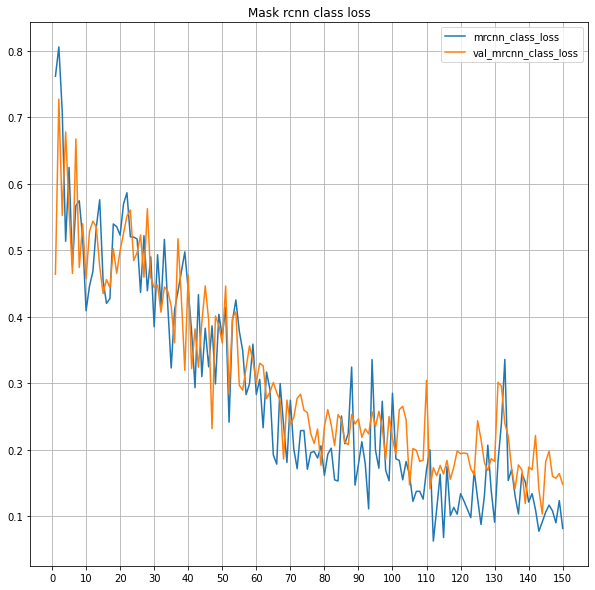
\includegraphics[width= 0.55\linewidth]{bab4/2. MRCNN_Class_Loss.png}
    \caption{Hasil \textit{Class Loss} Mask RCNN}
    \label{fig: Class Loss Mask RCNN}
  \end{center}
\end{figure}

Sedangkan pada metriks \textit{Loss Bounding Box Mask R-CNN} (gambar \ref{fig: Bounding Box Loss Mask RCNN})
awalnya memiliki nilai loss 0,63 namun perlahan lahan turun mendekati nilai stabil pada 0,17 setelah 
60 epoch. Parameter loss ini memiliki nilai terendah pada epoch 111 dengan nilai 0,1528. Tanda-tanda
\textit{overfitting} juga mulai terlihat setelah epoch 100, walaupun begitu nilai selisih antara loss
\textit{train} dan \textit{validation} tidak terlalu jauh hanya sekitar 0,05.

\begin{figure}[h!]
  \begin{center}
    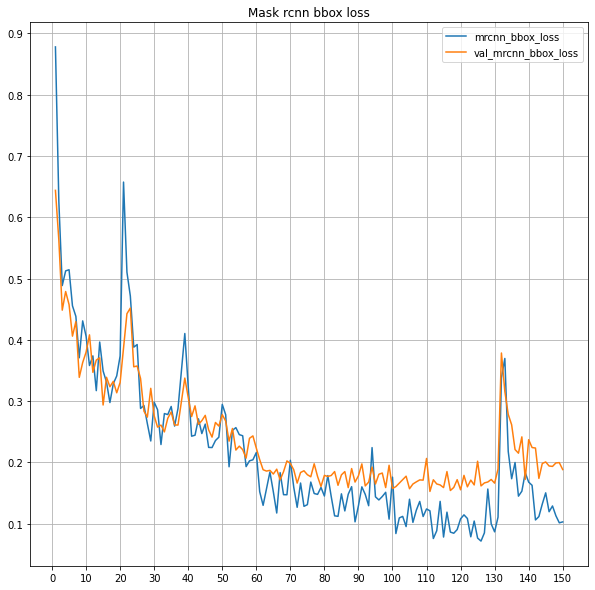
\includegraphics[width= 0.55\linewidth]{bab4/4. MRCNN_Bbox_Loss.png}
    \caption{Hasil \textit{Bounding Box Loss} Mask RCNN}
    \label{fig: Bounding Box Loss Mask RCNN}
  \end{center}
\end{figure}

Terakhir, metriks \textit{Loss Mask} digambarkan pada (gambar \ref{fig: Mask Loss Mask RCNN}).
Parameter ini merupakan parameter yang tercepat mencapai nilai stabil. Namun parameter loss ini memiliki
loss yang paling tinggi. Hal ini dikarenakan pembuatan mask diharapkan seakurat piksel segmentasi dataset,
namun untuk melakukan segmentasi secara akurat pada dataset pun merupakan hal yang sangat sulit dilakukan.
Nilai loss yang besar ini dapat memberikan masalah jika mask yang dibentuk sangat tidak sesuai dengan objek,
karena itu pengujian dengan test dataset sangat diperlukan untuk melihat performa model secara keseluruhan.

\begin{figure}[h!]
  \begin{center}
    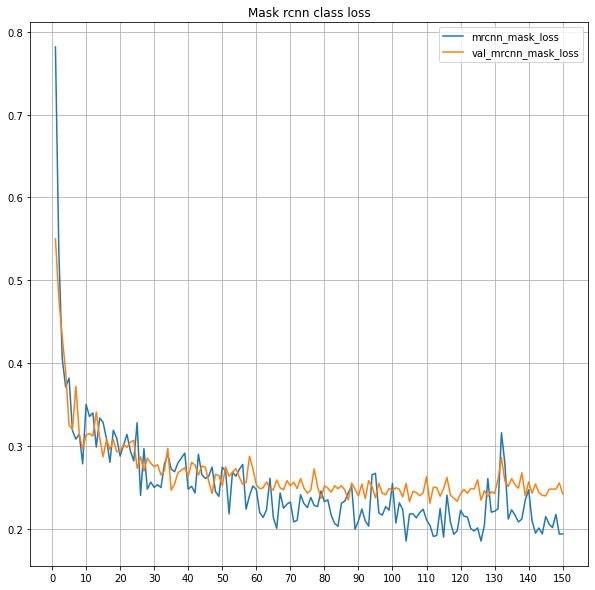
\includegraphics[width= 0.55\linewidth]{bab4/3. MRCNN_Mask_Loss.png}
    \caption{Hasil \textit{Mask Loss} Mask RCNN}
    \label{fig: Mask Loss Mask RCNN}
  \end{center}
\end{figure}

Berdasarkan parameter loss yang telah dipaparkan, maka peneliti memutuskan untuk mengambil model pada
epoch 124 karena memiliki nilai \textit{validation loss} terendah dari proses pelatihan. Model
pada epoch 124 memiliki detail \textit{loss} sebagai berikut.

\begin{table}
  \caption{Metriks Loss pada Model 124}
  \label{tab:MaskRCCN_Loss}
  \centering
  \begin{tabular}{ | l | l | }
    \hline
    \textbf{Parameter Model 124} & \textbf{Nilai} \\ \hline
    \textit{loss}             & 0,5877                   \\ \hline
    \textit{rpn class loss}    & 0,0076               \\ \hline
    \textit{rpn bounding box loss}             & 0,1102                  \\ \hline
    \textit{mrcnn class loss}             & 0,1683                   \\ \hline
    \textit{mrcnn bounding box loss}    & 0,1045                \\ \hline
    \textit{mrcnn mask loss}             & 0,1971                   \\ \hline

    \textit{val loss}             & 0,772                   \\ \hline
    \textit{val rpn class loss}    & 0,0069               \\ \hline
    \textit{val rpn bounding box loss}             & 0,1921                  \\ \hline
    \textit{val mrcnn class loss}             & 0,1620                   \\ \hline
    \textit{val mrcnn bounding box loss}    & 0,1634                \\ \hline
    \textit{val mrcnn mask loss}             & 0,2476                  \\ \hline
  \end{tabular}
\end{table}

\subsection{Hasil Pengujian pada Test Dataset}
Pengujian pada model epoch ke 124, dilakukan menggunakan test dataset yang mempunyai 134 gambar. Namun
sebelum model diuji secara keseluruhan, model akan diuji pada beberapa gambar. Hal ini dilakukan jika
hasil pada pengujian pada beberapa gambar menunjukkan nilai yang buruk, maka model tidak perlu diuji
dengan keseluruhan gambar.

\begin{figure}[h!]
  \begin{center}
    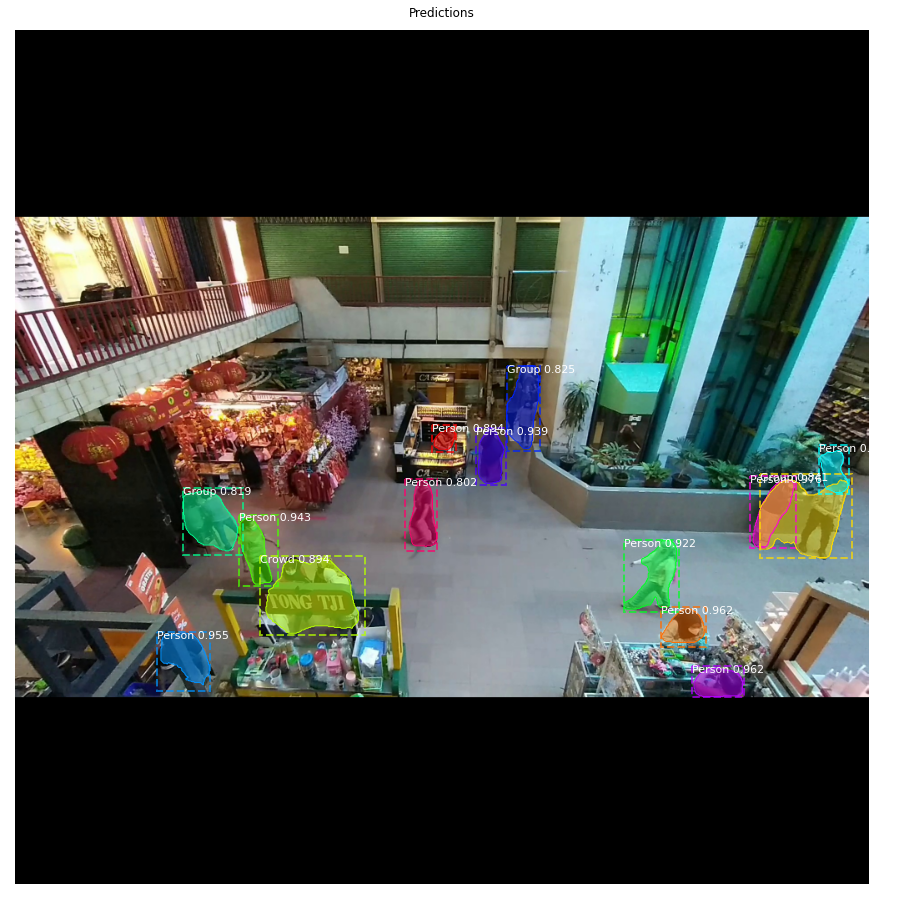
\includegraphics[width= 0.675\linewidth]{bab4/Contoh Hasil prediksi 1.png}
    \caption{Hasil Prediksi (1)}
    \label{fig: Predictions 1}
  \end{center}
\end{figure}

\begin{figure}[h!]
  \begin{center}
    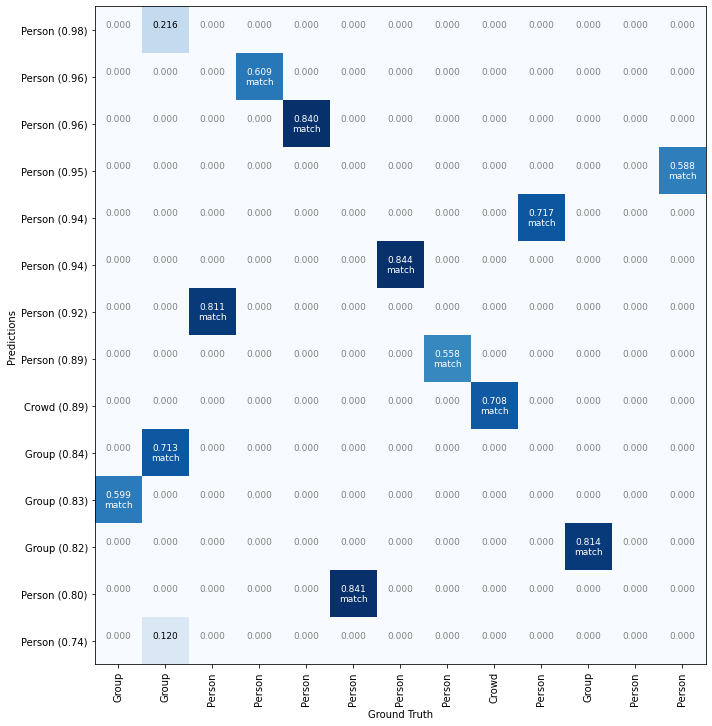
\includegraphics[width= 0.675\linewidth]{bab4/Contoh Hasil prediksi 1.6.png}
    \caption{Hasil Prediksi dan IoU (1)}
    \label{fig: Predictions and IoU}
  \end{center}
\end{figure}

\begin{figure}[h!]
  \begin{center}
    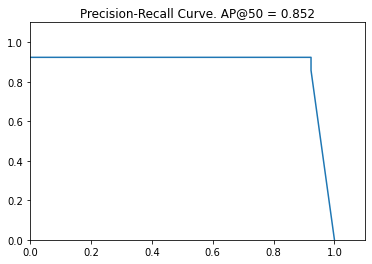
\includegraphics[width= 0.55\linewidth]{bab4/Contoh Hasil prediksi 1.5.png}
    \caption{Hasil Kurva Prediksi dan Recall (1)}
    \label{fig: line Predictions and IoU}
  \end{center}
\end{figure}

Gambar \ref{fig: Predictions and IoU} menunjukkan objek yang diprediksi dan \textit{ground truth} dimana
nilai prediksi dianggap benar jika IoU diatas 0,5. Dapat dilihat bahwa pada pengujian ini, 12 dari 14 objek
dapat diprediksi secara benar dan dengan \textit{confidence} di atas 70\%. Nilai \textit{confidence}
dapat dilihat pada label sebelah kiri, sebagai contoh Person(0,96) berarti, model yang diaplikasikan
mendeteksi suatu objek dengan nilai \textit{confidence} 96\% bahwa objek tersebut adalah objek kelas person.
Sedangkan nilai yang berwarna biru adalah nilai dari \textit{intersect over union} dimana jika nilai 
tersebut berada di atas nilai 0,5 maka dianggap prediksi benar.

Sedangkan grafik pada gambar \ref{fig: line Predictions and IoU} menunjukkan grafik hubungan antara
presisi dan \textit{recall} pada gambar yang diprediksi. Nilai pada x-axis menunjukkan nilai \textit{recall}
sedangkan nilai pada y-axis menunjukkan nilai presisi dan nilai \textit{threshold}. Gambar \ref{fig: line Predictions and IoU}
menunjukkan bahwa, saat diuji coba pada gambar tersebut, dengan threshold deteksi (\textit{confidence})
0,852, nilai presisinya ialah 0,852 dan nilai \textit{recall} adalah 0,92. Model ini dapat dikatakan model
yang bagus dalam mendeteksi gambar tersebut.

Kemudian saat diuji coba dengan gambar kedua, dapat dilihat bahwa model mendeteksi objek pada gambar
dengan baik. dengan \textit{threshold} 0,812, nilai presisi dan \textit{recall} pada model pun cukup
bagus. Deteksi yang dihasilkan pada uji coba gambar kedua ini pun dapat dihitung cukup memuaskan 
karena nilai \textit{confidence} di atas nilai 0,8. Walaupun ada satu objek kelas\textit{group} yang 
tidak terdeteksi, namun dari 8 objek yang ada, model dapat mendeteksi 7 objek dengan kelas yang benar
dan mayoritas objek yang dideteksi mempunyai nilai \textit{interference over union} di atas 0,7. terdapat
satu objek kelas yang memiliki \textit{interference over union} 0,693, namun saat dilihat pada gambar,
objek tersebut memiliki \textit{mask} yang cukup baik. Kemudian dapat dilihat juga bahwa model
dapat memprediksi objek \textit{person} yang hanya terlihat bagian kakinya, tentunya ini dapat dinilai
sebagai model yang cukup cerdas dalam memperhatikan fitur manusia. Hasil prediksi pada gambar
kedua dapat dilihat pada gambar \ref{fig: Predictions 2}. Sedangkan untuk nilai \textit{confidence} dan
nilai IoU dapat dilihat pada gambar \ref{fig: Predictions 2.6} dan kurva \textit{precission-recall} dapat 
dilihat pada gambar \ref{fig: Predictions 2.5}. Dengan hasil ini dapat disimpulkan secara sementara
bahwa model yang dibentuk memiliki kemampuan deteksi yang baik.

\begin{figure}[h!]
  \begin{center}
    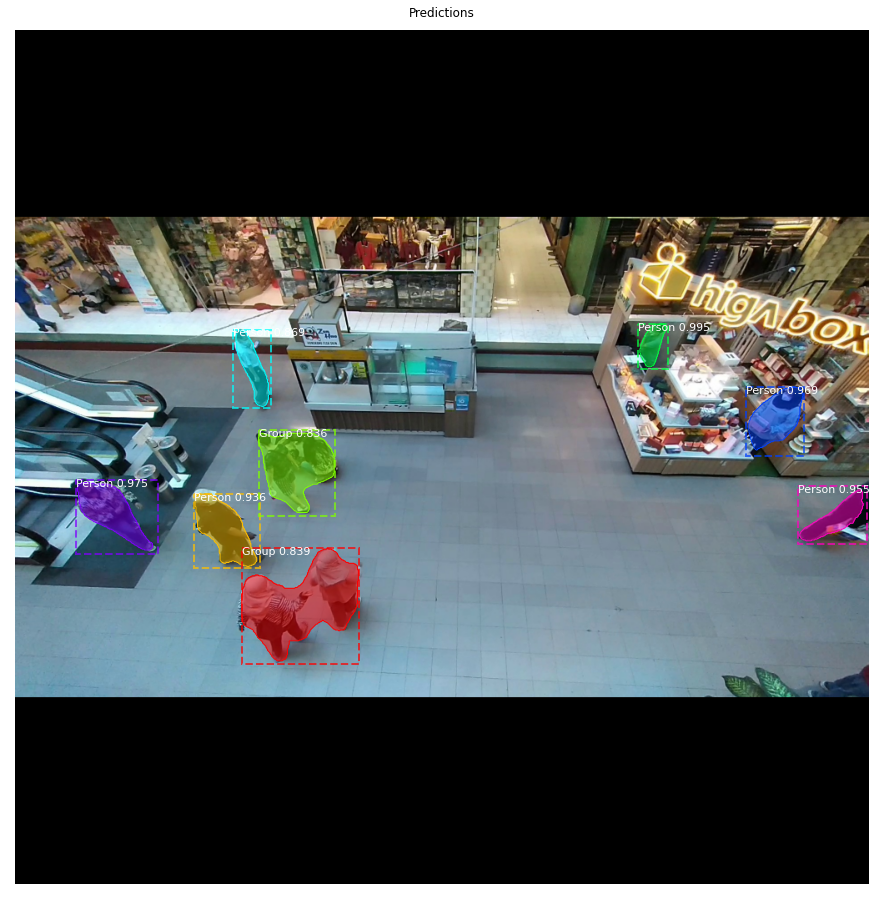
\includegraphics[width= 0.7\linewidth]{bab4/Contoh Hasil prediksi 3.png}
    \caption{Contoh Hasil Prediksi (2)}
    \label{fig: Predictions 2}
  \end{center}
\end{figure}

\begin{figure}[h!]
  \begin{center}
    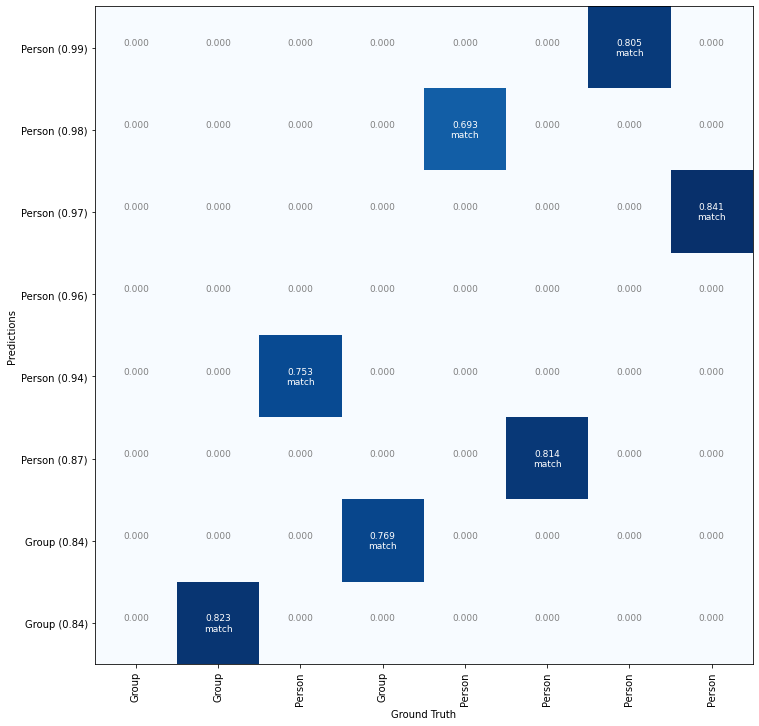
\includegraphics[width= 0.7\linewidth]{bab4/Contoh Hasil prediksi 3.6.png}
    \caption{Hasil Kurva Prediksi dan Recall (2)}
    \label{fig: Predictions 2.6}
  \end{center}
\end{figure}

\begin{figure}[h!]
  \begin{center}
    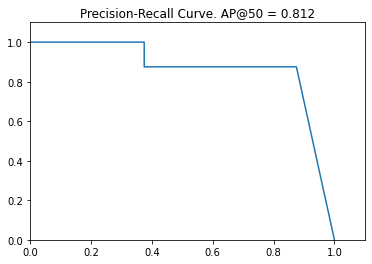
\includegraphics[width= 0.7\linewidth]{bab4/Contoh Hasil prediksi 3.5.png}
    \caption{Contoh Hasil Prediksi dan IoU(2)}
    \label{fig: Predictions 2.5}
  \end{center}
\end{figure}

\begin{figure}[h!]
  \begin{center}
    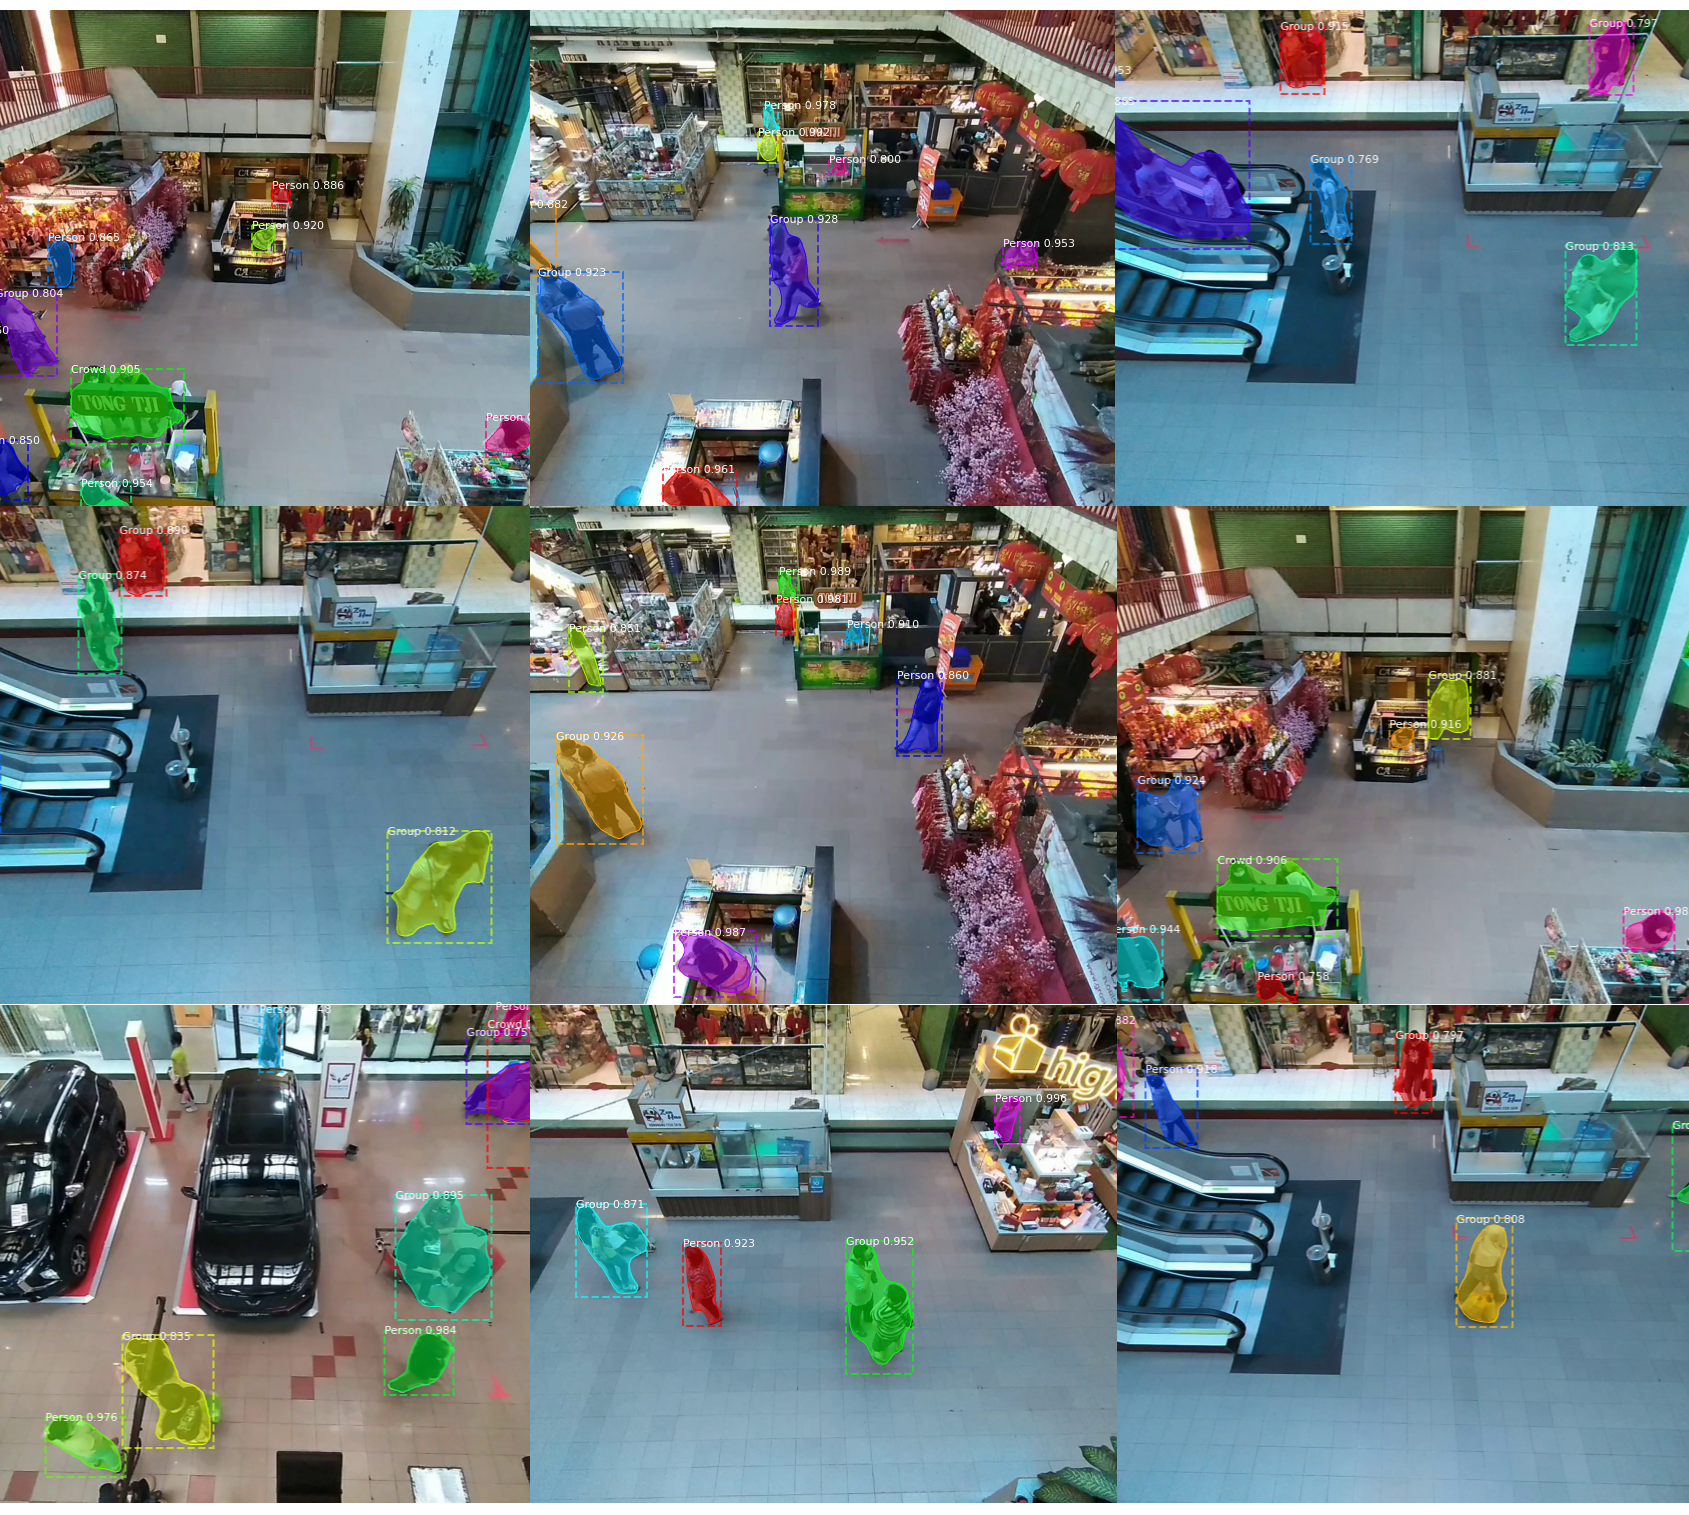
\includegraphics[width= 0.55\linewidth]{bab4/Hasil Test.png}
    \caption{Beberapa Hasil Deteksi pada Dataset Test}
    \label{fig: Test Dataset Result}
  \end{center}
\end{figure}

Setelah pengujian dengan beberapa gambar, maka pengujian dilakukan menggunakan seluruh test dataset.
Hasil dari pengujian divisualisasikan dengan \textit{confusion matrix} pada gambar \ref{fig: Conf Matrix Test}.
Perlu diketahui bahwa parameter deteksi adalah dimana model memiliki \textit{confidence} lebih dari 
70\% pada sebuah deteksi objek dan memiliki \textit{interference over union} lebih dari 50\%. Pada
\textit{confusion matrix} kita dapat mengetahui bahwa akurasi secara menyeluruh dari model yang dihasilkan adalah 88,79\%. 
Dari total 591 objek kelas \textit{person}, model dapat mendeteksi 531 objek kelas person yang benar.
Sedangkan dari total 296 objek dengan kelas \textit{group}, model dapat mendeteksi 261 objek kelas 
\textit{group} secara benar. Terakhir, dari total 32 objek kelas \textit{crowd}, terdapat 24 objek
kelas \textit{crowd} yang dideteksi dengan benar. Selain itu, tidak ada satupun objek dengan kelas 
\textit{person} dideteksi sebagai objek kelas \textit{crowd}

Dapat dilihat juga bahwa \textit{recall} pada objek kelas \textit{person} adalah 89,85\% dan memiliki
presisi sebesar 95,85\%. Selanjutnya pada objek kelas \textit{group}, \textit{recall} yang dihasilkan
adalah 88,17\% dengan presisi sebesar 79,33\%. Terakhir pada objek kelas \textit{crowd}, model memiliki
performa deteksi yang paling rendah dibandingkan kelas yang lainnya yaitu 75\% \textit{recall} dan
66,67\% pada presisi. Namun semua kelas \textit{crowd} terdeteksi sebagai kelas \textit{crowd} dan
\textit{group}. Tidak ada kelas \textit{crowd} yang terdeteksi sebagai kelas \textit{person} sehingga
kelas ini dapat dianggap sebagai terdeteksi sebagai parameter yang berbahaya dalam masa pandemi Covid-19.

\begin{figure}[h!]
  \begin{center}
    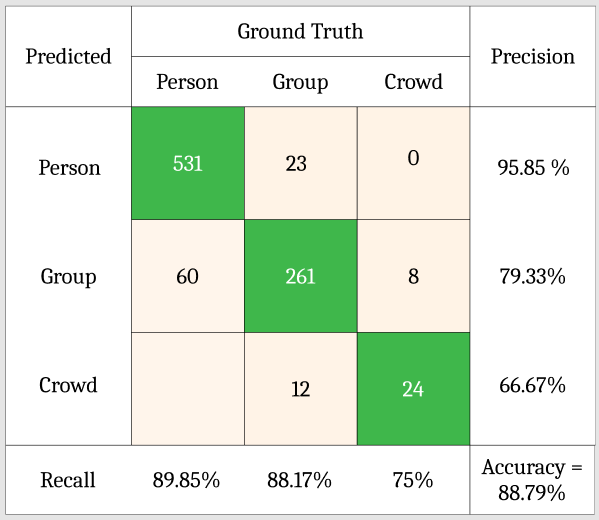
\includegraphics[width= 0.5\linewidth]{bab4/Confusion Matrix.png}
    \caption{\textit{Confusion Matrix} dari Hasil Prediksi Test Dataset}
    \label{fig: Conf Matrix Test}
  \end{center}
\end{figure}
